

%334% 
$$ asdasd $$
\chapter{Validação \& Verificação}


O desenvolvimento de softwares de simulação, seja utilizando o MEF ou não, é sempre acompanhado de uma bateria de testes, além de um procedimento de validação e verificação (V \& V), que garante, dentro de uma margem de abrangência do que se propõe, sua capacidade de reproduzir resultados concisos, sendo, então, um espelho da realidade.

Verificação, dentro desse contexto, é o procedimento pelo qual se evidencia a exata implementação do modelo matemático no próprio software, ou seja, a verificação que a modelagem programada é equivalente ao algoritmo matemático, dentro dos limites impostos pela aritmética computacional em relação às operações em ponto flutuante\footnote{No computador, os números ditos Reais ($\mathbb{R}$) são representandos por um ponto flutuante, que é uma forma discreta, pois os computadores são desenvolvidos em lógica booleana}. Já a validação, por sua vez, é o processo para determinar a acurácia que um modelo computacional possui de presentar a realidade, dentro dos limites que se propõe. Essas definições estão de acordo com o documento \emph{An Overview of the Guide for Verification and Validation
in Computational Solid Mechanics}, referente a norma ASME respectiva.

Por questões de simplificação, a verificação foi realizada por comparação com outro programa que realiza a mesma análise, o Abaqus, e a validação, por comparação com resultados analíticos, já consolidados experimentalmente.

\section{Verificação}

Para verificar os resultados foram utilizados seis sequências de comparação (três com o elemento tetraédrico, e três triangulares), nas quais aplicaram-se todas as condições de contorno (deslocamentos prescritos, carregamentos pontuais, em linhas e superficiais). Os resultados foram comparados com os obtidos no Abaqus, nas mesmas condições de contorno e geometrias, para deslocamentos nodais e tensões sobre os elementos. As geometrias empregadas foram simples, com malhas pouco refinadas, a fim de facilitar a comparação sobre todos os nós e elementos.

Os arquivos de verificação estão disponíveis no repositório do projeto, no pasta \emph{verification}, na qual constam os arquivos de entrada do Abaqus (\emph{.cae}) e do GID (\emph{.gid}), além dos arquivos respectivos arquivos de saída, (\emph{.rpt} e \emph{.post.res})

Em todos os casos, definiu-se o aço ASIS 4340 como material, cujas características físicas empregadas aqui foram: $E = 210 \text{GPa}$ (módulo de elasticidade) e $\nu = 0.3$ (coeficiente de Poisson).

Primeiramente, o problema é definido no Abaqus, para depois ser exportado para o GID, a fim de se manter tanto a geometria como a malha e, principalmente, as identificações dos nós e elementos, o que facilitada a comparação dos resultados. O procedimento empregado em todos os casos foi o seguinte:

\begin{enumerate}
    \item Definição do problema no Abaqus (\emph{.cae});
    \begin{enumerate}
        \item Construção da geometria;
        \item Definição do material (AISI 4340 STEEL);
        \item Construção da malha;
        \item Definição das condições de contorno;
    \end{enumerate} 
    \item Execução da análise;
    \item Exportação dos resultados para um arquivo de texto (\emph{.rpt});
    \begin{enumerate}
        \item utilização da ferramenta \emph{probe} sobre os nós (deslocamentos nodais);
        \item utilização da ferramenta \emph{probe} sobre os elementos (componentes das tensões e tensão de von Mises);
    \end{enumerate}
    \item Importação do arquivo de \emph{input} no GID (\emph{.inp});
    \item Definição do problema no GID;
    \begin{enumerate}
        \item Definição do material (AISI 4340 STEEL);
        \item Definição das condições de contorno;
    \end{enumerate}
    \item Execução da análise;
    \item Exportação do arquivo de resultados (\emph{.post.res});
    \item Comparação dos resultados.
\end{enumerate}

\subsection{Casos tridimensionais (elemento tetraédrico)}

\begin{figure}
    \centering
    \caption{O cubo unitário.}
    \begin{subfigure}[b]{0.45\textwidth}
        \centering
        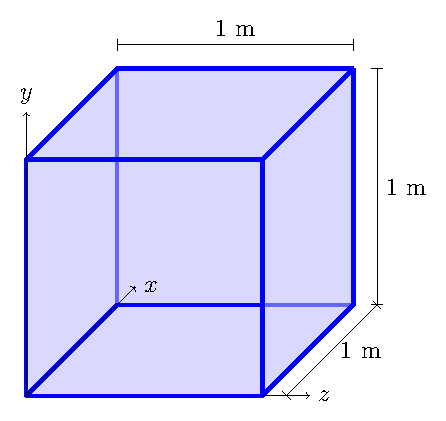
\includegraphics[page=1]{Figuras/verificacao_cubo.pdf}
        \caption{Geometria}
        \label{fig:verificacao_cubo_1}
    \end{subfigure}
    \begin{subfigure}[b]{0.45\textwidth}
        \centering
        \includegraphics[page=2]{Figuras/verificacao_cubo.pdf}
        \caption{Malha}
        \label{fig:verificacao_cubo_2}
    \end{subfigure}
\end{figure}

Nos casos tridimensionais foi empregado a geometria de um cubo unitário, conforme a figura \ref{fig:verificacao_cubo_1}, com a malha descrita na tabela \ref{tab:nos_cubo} (figura \ref{fig:verificacao_cubo_2}) e conectividade na tabela \ref{tab:elementos_cubo}. A face formada pelos nós $3$, $4$, $7$ e $6$ foi engastada, e as demais condições de contorno foram aplicadas nas seguintes sequências:

\begin{enumerate}
    \item Carregamento superficial (figura \ref{fig:verificacao_cubo_3}), resultados nas tabelas \ref{tab:verificacao_cubo_1_deslocamentos} e \ref{tab:verificacao_cubo_1_tensoes};
    \item Carregamento pontual (figura \ref{fig:verificacao_cubo_4}), resultados nas tabelas \ref{tab:verificacao_cubo_2_deslocamentos} e \ref{tab:verificacao_cubo_2_tenoes};
    \item Deslocamento prescrito (figura \ref{fig:verificacao_cubo_5}), resultados nas tabelas \ref{tab:verificacao_cubo_3_deslocamentos} e \ref{tab:verificacao_cubo_3_tenoes}.
\end{enumerate}

\begin{table}
    \centering
    \caption{Descrição dos nós para a malha do cubo unitário.}
    \begin{tabular}{c | c c c}
        \toprule
        \textbf{Nó} & \textbf{x} [m]  & \textbf{y}  [m]  & \textbf{z}  [m]  \\
        \midrule
        1 & 1.000000e+00 & 1.000000e+00 & 1.000000e+00 \\
        2 & 1.000000e+00 & 0.000000e+00 & 1.000000e+00 \\
        3 & 1.000000e+00 & 0.000000e+00 & 0.000000e+00 \\
        4 & 1.000000e+00 & 1.000000e+00 & 0.000000e+00 \\
        5 & 0.000000e+00 & 0.000000e+00 & 1.000000e+00 \\
        6 & 0.000000e+00 & 0.000000e+00 & 0.000000e+00 \\
        7 & 0.000000e+00 & 1.000000e+00 & 0.000000e+00 \\
        8 & 0.000000e+00 & 1.000000e+00 & 1.000000e+00 \\
        9 & 4.929074e-01 & 5.337674e-01 & 5.471772e-01 \\
        \bottomrule
    \end{tabular}
    \label{tab:nos_cubo}
\end{table}

\begin{table}
    \centering
    \caption{conectividade dos elementos na malha do cubo unitário.}
    \begin{tabular}{c | c c c c}
        \toprule
        \textbf{Elemento} & \textbf{Nó 1} & \textbf{Nó 2} & \textbf{Nó 3}  & \textbf{Nó 4} \\
        \midrule
        1 & 2 & 6 & 5 & 9 \\
        2 & 9 & 6 & 5 & 7 \\
        3 & 7 & 9 & 8 & 5 \\
        4 & 6 & 7 & 9 & 3 \\
        5 & 4 & 9 & 1 & 8 \\
        6 & 3 & 4 & 9 & 1 \\
        7 & 3 & 7 & 9 & 4 \\
        8 & 3 & 9 & 2 & 1 \\
        9 & 5 & 9 & 8 & 2 \\
        10 & 9 & 2 & 1 & 8 \\
        11 & 6 & 9 & 2 & 3 \\
        12 & 7 & 9 & 4 & 8 \\
        \bottomrule
    \end{tabular}
    \label{tab:elementos_cubo}
\end{table}

\begin{figure}
    \centering
    \caption{Condições de contorno para os casos tridimensionais.}
    \begin{subfigure}[b]{0.45\textwidth}
        \centering
        \includegraphics[page=3]{Figuras/verificacao_cubo.pdf}
        \caption{Carregamento superficial}
        \label{fig:verificacao_cubo_3}
    \end{subfigure}
    \begin{subfigure}[b]{0.45\textwidth}
        \centering
        \includegraphics[page=4]{Figuras/verificacao_cubo.pdf}
        \caption{Carga concentrada}
        \label{fig:verificacao_cubo_4}
    \end{subfigure}
    \begin{subfigure}[b]{0.45\textwidth}
        \centering
        \includegraphics[page=5]{Figuras/verificacao_cubo.pdf}
        \caption{Deslocamento prescrito}
        \label{fig:verificacao_cubo_5}
    \end{subfigure}
\end{figure}

\begin{table}
    \centering
    \caption{Deslocamentos nodais para o primeiro caso tridimensional.}
    \begin{tabular}{c | c c c }
        \toprule
        \multirow{2}{*}{\textbf{Nó}} & \multicolumn{3}{c}{\textbf{PHILLIPO.jl}}  \\
                                     & \textbf{x} [m] & \textbf{y} [m] & \textbf{z} [m]\\                            
        \midrule
        1 & $8.65925 \times 10^{-8}$ & $-8.92024 \times 10^{-6}$ & $1.71092 \times 10^{-6}$ \\
        2 & $2.34872 \times 10^{-7}$ & $-7.50586 \times 10^{-6}$ & $-2.45344 \times 10^{-6}$ \\
        3 & 0.0 & 0.0 & 0.0 \\
        4 & 0.0 & 0.0 & 0.0 \\
        5 & $-4.97641 \times 10^{-7}$ & $-7.52208 \times 10^{-6}$ & $-1.51181 \times 10^{-6}$ \\
        6 & 0.0 & 0.0 & 0.0 \\
        7 & 0.0 & 0.0 & 0.0 \\
        8 & $-2.34375\times 10^{-7}$ & $-1.04911 \times 10^{-5}$ & $3.58197 \times 10^{-6}$ \\
        9 & $-1.43153 \times 10^{-7}$ & $-4.38813 \times 10^{-6}$ & $1.65793 \times 10^{-7}$ \\
        \bottomrule
    \end{tabular}
    \label{tab:verificacao_cubo_1_deslocamentos}
\end{table}

\begin{table}
    \centering
    \caption{Tensões sobre os elementos para o primeiro caso tridimensional.}

    \resizebox{\textwidth}{!}{
    \begin{tabular}{c | c c c c c c}
        \toprule
        \multirow{2}{*}{\textbf{ID}} & \multicolumn{6}{c}{\textbf{PHILLIPO.jl} [Pa]}  \\
                                           & \textbf{$\sigma_x$} & \textbf{$\sigma_y$} & \textbf{$\sigma_z$} & \textbf{$\sigma_{xy}$} & \textbf{$\sigma_{xz}$} & \textbf{$\sigma_{zy}$}\\                            
        \midrule
        1 & $-3.96885 \times 10^4$ & $-2.42821 \times 10^5$ & $-4.02234 \times 10^5$ & $-3.37838 \times 10^4$ & $-3.87057 \times 10^5$ & $-1.16248 \times 10^5$ \\
        2 & $-1.09096 \times 10^5$ & $-1.51419 \times 10^5$ & $-3.95636 \times 10^5$ & $-4.46066 \times 10^4$ & $-6.07553 \times 10^5$ & $1.22526 \times 10^5$ \\
        3 & $1.36097 \times 10^5$ & $-3.78867 \times 10^5$ & $6.79384 \times 10^5$ & $1.60388 \times 10^4$ & $-4.35943 \times 10^5$ & $7.62264 \times 10^4$ \\
        4 & $3.67093 \times 10^4$ & $3.67093 \times 10^4$ & $8.56550 \times 10^4$ & $0.00000$ & $-6.47735 \times 10^5$ & $-2.11311 \times 10^4$ \\
        5 & $-3.70490 \times 10^4$ & $-5.35656 \times 10^5$ & $1.87482 \times 10^5$ & $1.31695 \times 10^5$ & $-4.22653 \times 10^5$ & $-1.44130 \times 10^5$ \\
        6 & $3.13504 \times 10^5$ & $2.52807 \times 10^5$ & $5.29187 \times 10^5$ & $-7.84963 \times 10^4$ & $-7.20481 \times 10^5$ & $1.29700 \times 10^5$ \\
        7 & $3.67093 \times 10^4$ & $3.67093 \times 10^4$ & $8.56550 \times 10^4$ & $0.00000$ & $-6.47735 \times 10^5$ & $-2.11311 \times 10^4$ \\
        8 & $-3.61274 \times 10^5$ & $-6.51080 \times 10^5$ & $-8.18929 \times 10^5$ & $-8.74518 \times 10^4$ & $-2.69891 \times 10^5$ & $1.32782 \times 10^5$ \\
        9 & $1.77784 \times 10^3$ & $-5.96175 \times 10^5$ & $8.93419 \times 10^4$ & $2.25736 \times 10^4$ & $-4.28830 \times 10^5$ & $-4.98169 \times 10^4$ \\
        10 & $6.71645 \times 10^4$ & $-2.13160 \times 10^5$ & $2.12365 \times 10^5$ & $1.14907 \times 10^5$ & $-4.96502 \times 10^5$ & $-1.26844 \times 10^5$ \\
        11 & $-3.61046 \times 10^5$ & $-4.46115 \times 10^5$ & $-7.57371 \times 10^5$ & $-4.11090 \times 10^4$ & $-3.78014 \times 10^5$ & $1.89704 \times 10^4$ \\
        12 & $8.25382 \times 10^4$ & $-3.86038 \times 10^5$ & $6.61165 \times 10^5$ & $2.58282 \times 10^3$ & $-5.36544 \times 10^5$ & $-1.89303 \times 10^4$ \\
        \bottomrule
    \end{tabular}}
    \label{tab:verificacao_cubo_1_tensoes}
\end{table}


\begin{table}
    \centering
    \caption{Deslocamentos nodais para o segundo caso tridimensional.}
    \begin{tabular}{c | c c c }
        \toprule
        \multirow{2}{*}{\textbf{Nó}} & \multicolumn{3}{c}{\textbf{PHILLIPO.jl}}  \\
                                     & \textbf{x} [m] & \textbf{y} [m] & \textbf{z} [m]\\                            
        \midrule
        1 & $1.02738 \times 10^{-6}$ & $-2.02588 \times 10^{-5}$ & $3.00251 \times 10^{-6}$ \\
        2 & $-4.34358 \times 10^{-7}$ & $-1.56996 \times 10^{-5}$ & $-4.85199 \times 10^{-6}$ \\
        3 & $0.0$ & $0.0$ & $0.0$ \\
        4 & $0.0$ & $0.0$ & $0.0$ \\
        5 & $-1.19159 \times 10^{-6}$ & $-1.38869 \times 10^{-5}$ & $-2.90123 \times 10^{-6}$ \\
        6 & $0.0$ & $0.0$ & $0.0$ \\
        7 & $0.0$ & $0.0$ & $0.0$ \\
        8 & $4.4546 \times 10^{-7}$ & $-1.89878 \times 10^{-5}$ & $6.81349 \times 10^{-6}$ \\
        9 & $-3.03331 \times 10^{-7}$ & $-8.53913 \times 10^{-6}$ & $1.49066 \times 10^{-7}$ \\
        \bottomrule
    \end{tabular}
    \label{tab:verificacao_cubo_2_deslocamentos}
\end{table}

\begin{table}
    \centering
    \caption{Tensões sobre os elementos para o segundo caso tridimensional.}

    \resizebox{\textwidth}{!}{
    \begin{tabular}{c | c c c c c c}
        \toprule
        \multirow{2}{*}{\textbf{ID}} & \multicolumn{6}{c}{\textbf{PHILLIPO.jl} [Pa]}  \\
                                           & \textbf{$\sigma_x$} & \textbf{$\sigma_y$} & \textbf{$\sigma_z$} & \textbf{$\sigma_{xy}$} & \textbf{$\sigma_{xz}$} & \textbf{$\sigma_{zy}$}\\                            
        \midrule
        1 & $-1.48107 \times 10^5$ & $-2.84665 \times 10^5$ & $-7.39090 \times 10^5$ & $-1.50128 \times 10^5$ & $-7.13362 \times 10^5$ & $-2.53806 \times 10^5$ \\
        2 & $-1.51519 \times 10^5$ & $-2.65791 \times 10^5$ & $-7.34452 \times 10^5$ & $-1.54118 \times 10^5$ & $-1.12164 \times 10^6$ & $1.88313 \times 10^5$ \\
        3 & $3.31474 \times 10^5$ & $-5.63353 \times 10^5$ & $1.36127 \times 10^6$ & $4.57622 \times 10^4$ & $-7.48975 \times 10^5$ & $1.91682 \times 10^5$ \\
        4 & $3.30055 \times 10^4$ & $3.30055 \times 10^4$ & $7.70128 \times 10^4$ & $0.0$ & $-1.26047 \times 10^6$ & $-4.47749 \times 10^4$ \\
        5 & $3.41582 \times 10^4$ & $-7.18663 \times 10^5$ & $4.25177 \times 10^5$ & $-3.84442 \times 10^3$ & $-1.04271 \times 10^6$ & $-2.24829 \times 10^5$ \\
        6 & $8.46258 \times 10^5$ & $5.70548 \times 10^5$ & $1.05557 \times 10^6$ & $-4.05526 \times 10^5$ & $-1.63629 \times 10^6$ & $3.20919 \times 10^5$ \\
        7 & $3.30055 \times 10^4$ & $3.30055 \times 10^4$ & $7.70128 \times 10^4$ & $0.0$ & $-1.26047 \times 10^6$ & $-4.47749 \times 10^4$ \\
        8 & $-6.68634 \times 10^5$ & $-1.67458 \times 10^6$ & $-1.72188 \times 10^6$ & $-2.77724 \times 10^5$ & $-6.33643 \times 10^5$ & $1.86079 \times 10^5$ \\
        9 & $-8.99318 \times 10^4$ & $-1.03624 \times 10^6$ & $2.06398 \times 10^5$ & $-1.41868 \times 10^4$ & $-8.14231 \times 10^5$ & $-9.35646 \times 10^4$ \\
        10 & $-8.71417 \times 10^4$ & $-9.17625 \times 10^5$ & $2.19806 \times 10^5$ & $1.54039 \times 10^4$ & $-9.61902 \times 10^5$ & $-2.44647 \times 10^5$ \\
        11 & $-5.76185 \times 10^5$ & $-5.60648 \times 10^5$ & $-1.35997 \times 10^6$ & $-9.93562 \times 10^3$ & $-8.43752 \times 10^5$ & $-3.50827 \times 10^4$ \\
        12 & $3.44607 \times 10^5$ & $-2.96558 \times 10^5$ & $1.44525 \times 10^6$ & $9.47744 \times 10^4$ & $-9.13586 \times 10^5$ & $3.59795 \times 10^4$ \\
        \bottomrule
    \end{tabular}}
    \label{tab:verificacao_cubo_2_tenoes}
\end{table}


\begin{table}
    \centering
    \caption{Deslocamentos nodais para o terceiro caso tridimensional.}
    \begin{tabular}{c | c c c }
        \toprule
        \multirow{2}{*}{\textbf{Nó}} & \multicolumn{3}{c}{\textbf{PHILLIPO.jl}}  \\
                                     & \textbf{x} [m] & \textbf{y} [m] & \textbf{z} [m]\\                            
        \midrule
        1 & $0.00000 \times 10^{0}$ & $0.00000 \times 10^{0}$ & $0.10000 \times 10^{0}$ \\
        2 & $-5.32004 \times 10^{-3}$ & $-1.33670 \times 10^{-3}$ & $-1.85191 \times 10^{-3}$ \\
        3 & $0.00000 \times 10^{0}$ & $0.00000 \times 10^{0}$ & $0.00000 \times 10^{0}$ \\
        4 & $0.00000 \times 10^{0}$ & $0.00000 \times 10^{0}$ & $0.00000 \times 10^{0}$ \\
        5 & $1.45540 \times 10^{-2}$ & $1.22280 \times 10^{-2}$ & $2.39641 \times 10^{-2}$ \\
        6 & $0.00000 \times 10^{0}$ & $0.00000 \times 10^{0}$ & $0.00000 \times 10^{0}$ \\
        7 & $0.00000 \times 10^{0}$ & $0.00000 \times 10^{0}$ & $0.00000 \times 10^{0}$ \\
        8 & $0.00000 \times 10^{0}$ & $0.00000 \times 10^{0}$ & $0.10000 \times 10^{0}$ \\
        9 & $1.19228 \times 10^{-3}$ & $1.15650 \times 10^{-2}$ & $2.80404 \times 10^{-2}$ \\
        \bottomrule
    \end{tabular}
    \label{tab:verificacao_cubo_3_deslocamentos}
\end{table}

\begin{table}
    \centering
    \caption{Tensões sobre os elementos para o terceiro caso tridimensional.}

    \resizebox{\textwidth}{!}{
    \begin{tabular}{c | c c c c c c}
        \toprule
        \multirow{2}{*}{\textbf{ID}} & \multicolumn{6}{c}{\textbf{PHILLIPO.jl} [Pa]}  \\
                                           & \textbf{$\sigma_x$} & \textbf{$\sigma_y$} & \textbf{$\sigma_z$} & \textbf{$\sigma_{xy}$} & \textbf{$\sigma_{xz}$} & \textbf{$\sigma_{zy}$}\\                            
        \midrule
        1 & $-9.09572 \times 10^7$ & $6.61804 \times 10^9$ & $6.99059 \times 10^9$ & $-6.37915 \times 10^8$ & $5.17203 \times 10^9$ & $-9.09626 \times 10^8$ \\
        2 & $-9.80149 \times 10^8$ & $1.239 \times 10^9$ & $5.11012 \times 10^9$ & $7.98683 \times 10^8$ & $9.87649 \times 10^8$ & $3.62163 \times 10^9$ \\
        3 & $7.42606 \times 10^9$ & $7.28382 \times 10^9$ & $2.5413 \times 10^{10}$ & $-2.14641 \times 10^8$ & $6.14136 \times 10^9$ & $1.43759 \times 10^9$ \\
        4 & $6.2086 \times 10^9$ & $6.2086 \times 10^9$ & $1.44867 \times 10^{10}$ & $0.0$ & $1.70712 \times 10^9$ & $1.75993 \times 10^8$ \\
        5 & $9.11014 \times 10^9$ & $5.10314 \times 10^9$ & $2.5264 \times 10^{10}$ & $-2.06548 \times 10^8$ & $4.62152 \times 10^9$ & $0.0$ \\
        6 & $1.14507 \times 10^{10}$ & $1.18305 \times 10^{10}$ & $2.79844 \times 10^{10}$ & $-1.84206 \times 10^9$ & $0.0$ & $4.24913 \times 10^9$ \\
        7 & $6.2086 \times 10^9$ & $6.2086 \times 10^9$ & $1.44867 \times 10^{10}$ & $0.0$ & $1.70712 \times 10^9$ & $1.75993 \times 10^8$ \\
        8 & $-7.66859 \times 10^8$ & $-1.48395 \times 10^8$ & $-6.63477 \times 10^8$ & $-1.41522 \times 10^9$ & $8.11854 \times 10^9$ & $3.60189 \times 10^9$ \\
        9 & $-7.36171 \times 10^8$ & $4.98949 \times 10^8$ & $1.0959 \times 10^{10}$ & $-2.27113 \times 10^9$ & $3.90283 \times 10^9$ & $-2.83479 \times 10^9$ \\
        10 & $6.70973 \times 10^9$ & $6.92566 \times 10^9$ & $1.54401 \times 10^{10}$ & $4.29695 \times 10^8$ & $6.05251 \times 10^9$ & $-6.55085 \times 10^8$ \\
        11 & $2.56666 \times 10^9$ & $6.28802 \times 10^9$ & $2.2675 \times 10^9$ & $6.20905 \times 10^8$ & $4.28842 \times 10^9$ & $-4.29695 \times 10^8$ \\
        12 & $9.11014 \times 10^9$ & $5.10314 \times 10^9$ & $2.5264 \times 10^{10}$ & $-2.06548 \times 10^8$ & $4.62152 \times 10^9$ & $0.0$ \\
        \bottomrule
    \end{tabular}}
    \label{tab:verificacao_cubo_3_tenoes}
\end{table}



Em todas as sequências de comparação para o caso tridimensionais, os resultados exportados do Abaqus convergiram com os produzidos por PHILLIPO, com exceção dos deslocamentos prescritos, que não são definidos exatamente zero nos engastes, o que pode ser devido ao procedimento de solução do sistema no Abaqus, por algum método iterativo ou de penalização, porém essa diferença é desprezível.

Destes modo, fica demonstrado que algoritmo matemático do ME foi implementado corretamente nessas condições. 

\subsection{Casos bidimensionais (elemento triangular)}

Nos casos bidimensionais foi empregado a geometria de um quadrado unitário, conforme a figura \ref{fig:verificacao_quadrado_1}, com a malha descrita na tabela \ref{tab:nos_quadrado} (figura \ref{fig:verificacao_cubo_2}) e conectividade na tabela \ref{tab:elementos_quadrado}. A fronteira formada pelos nós $1$ e $3$, foi engastada, e as demais condições de contorno foram aplicadas nas seguintes sequências, dentro da análise do EPT:

\begin{enumerate}
    \item Carregamento em linha (figura \ref{fig:verificacao_quadrado_3}), resultados nas tabelas \ref{tab:verificacao_quadrado_1_deslocamentos} e \ref{tab:verificacao_quadrado_1_tensoes};
    \item Carregamento pontual (figura \ref{fig:verificacao_quadrado_4}), resultados nas tabelas \ref{tab:verificacao_quadrado_2_deslocamentos} e \ref{tab:verificacao_quadrado_2_tenoes};
    \item Deslocamento prescrito (figura \ref{fig:verificacao_cubo_5}) resultados nas tabelas \ref{tab:verificacao_quadrado_3_deslocamentos} e \ref{tab:verificacao_quadrado_3_tenoes}.
\end{enumerate}

\begin{table}
    \centering
    \caption{Descrição dos nós para a malha do quadrado unitário.}
    \begin{tabular}{c | c c}
        \toprule
        \textbf{Nó} & \textbf{x} [m]  & \textbf{y}  [m] \\
        \midrule
        1 & 0.000000e+00 & 0.000000e+00 \\
        2 & 1.000000e+00 & 0.000000e+00 \\
        3 & 0.000000e+00 & 1.000000e+00 \\
        4 & 1.000000e+00 & 1.000000e+00 \\
        \bottomrule
    \end{tabular}
    \label{tab:nos_quadrado}
\end{table}

\begin{table}
    \centering
    \caption{conectividade dos elementos na malha do quadrado unitário.}
    \begin{tabular}{c | c c c}
        \toprule
        \textbf{Elemento} & \textbf{Nó 1} & \textbf{Nó 2} & \textbf{Nó 3} \\
        \midrule
        1 & 1 & 2 & 4 \\
        2 & 4 & 3 & 1 \\
        \bottomrule
    \end{tabular}
    \label{tab:elementos_quadrado}
\end{table}


\begin{figure}
    \centering
    \caption{O quadrado unitário.}
    \begin{subfigure}[b]{0.45\textwidth}
        \centering
        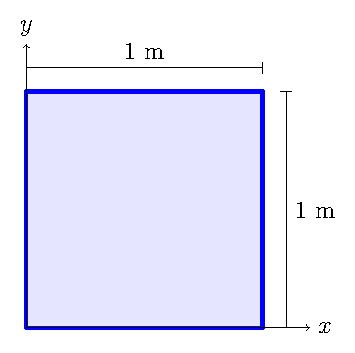
\includegraphics[page=1]{Figuras/verificacao_quadrado.pdf}
        \caption{Geometria}
        \label{fig:verificacao_quadrado_1}
    \end{subfigure}
    \begin{subfigure}[b]{0.45\textwidth}
        \centering
        \includegraphics[page=2]{Figuras/verificacao_quadrado.pdf}
        \caption{Malha}
        \label{fig:verificacao_quadrado_2}
    \end{subfigure}
\end{figure}

\begin{figure}
    \centering
    \caption{Condições de contorno para os casos bidimensionais.}
    \begin{subfigure}[b]{0.45\textwidth}
        \centering
        \includegraphics[page=3]{Figuras/verificacao_quadrado.pdf}
        \caption{Carregamento em linha}
        \label{fig:verificacao_quadrado_3}
    \end{subfigure}
    \begin{subfigure}[b]{0.45\textwidth}
        \centering
        \includegraphics[page=4]{Figuras/verificacao_quadrado.pdf}
        \caption{Carga concentrada}
        \label{fig:verificacao_quadrado_4}
    \end{subfigure}
    \begin{subfigure}[b]{0.45\textwidth}
        \centering
        \includegraphics[page=5]{Figuras/verificacao_quadrado.pdf}
        \caption{Deslocamento prescrito}
        \label{fig:verificacao_quadrado_5}
    \end{subfigure}
\end{figure}


\begin{table}
    \centering
    \caption{Deslocamentos nodais para o primeiro caso bidimensionais.}
    \begin{tabular}{c | c c c }
        \toprule
        \multirow{2}{*}{\textbf{Nó}} & \multicolumn{2}{c}{\textbf{PHILLIPO.jl}}  \\
                                     & \textbf{x} [m] & \textbf{y} [m] \\                            
        \midrule
        1 & 0.0 & 0.0 \\
        2 & $-1.15402\times10^{-6}$ & $-6.94059\times10^{-6}$ \\
        3 & 0.0 & 0.0 \\
        4 & $1.50022\times10^{-6}$ & $-8.09460\times10^{-6}$ \\
        \bottomrule
    \end{tabular}
    \label{tab:verificacao_quadrado_1_deslocamentos}
\end{table}

\begin{table}
    \centering
    \caption{Tensões sobre os elementos para o primeiro caso tridimensional.}
    \begin{tabular}{c | c c c}
        \toprule
        \multirow{2}{*}{\textbf{ID}} & \multicolumn{3}{c}{\textbf{PHILLIPO.jl} [Pa]}  \\
                                           & \textbf{$\sigma_x$} & \textbf{$\sigma_y$} & \textbf{$\sigma_{xy}$} \\                            
        \midrule
        1 & $-3.46205\times10^{5}$ & $-3.46205\times10^{5}$ & $-3.46205\times10^{5}$ \\
        2 & $3.46205\times10^{5}$ & $1.03862\times10^{5}$ & $-6.53794\times10^{5}$ \\
        \bottomrule
    \end{tabular}
    \label{tab:verificacao_quadrado_1_tensoes}
\end{table}


\begin{table}
    \centering
    \caption{Deslocamentos nodais para o segundo caso bidimensionais.}
    \begin{tabular}{c | c c c }
        \toprule
        \multirow{2}{*}{\textbf{Nó}} & \multicolumn{2}{c}{\textbf{PHILLIPO.jl}}  \\
                                     & \textbf{x} [m] & \textbf{y} [m] \\                            
        \midrule
        1 & 0.0 & 0.0 \\
        2 & $-1.15402\times10^{-6}$ & $-6.94059\times10^{-6}$ \\
        3 & 0.0 & 0.0 \\
        4 & $1.50022\times10^{-6}$ & $-8.09460\times10^{-6}$ \\
        \bottomrule
    \end{tabular}
    \label{tab:verificacao_quadrado_2_deslocamentos}
\end{table}

\begin{table}
    \centering
    \caption{Tensões sobre os elementos para o segundo caso tridimensional.}
    \begin{tabular}{c | c c c}
        \toprule
        \multirow{2}{*}{\textbf{ID}} & \multicolumn{3}{c}{\textbf{PHILLIPO.jl} [Pa]}  \\
                                           & \textbf{$\sigma_x$} & \textbf{$\sigma_y$} & \textbf{$\sigma_{xy}$} \\                            
        \midrule
        1 & $-3.46205\times10^{5}$ & $-3.46205\times10^{5}$ & $-3.46205\times10^{5}$ \\
        2 & $3.46205\times10^{5}$ & $1.03862\times10^{5}$ & $-6.53794\times10^{5}$ \\
        \bottomrule
    \end{tabular}
    \label{tab:verificacao_quadrado_2_tensoes}
\end{table}


\begin{table}
    \centering
    \caption{Deslocamentos nodais para o terceiro caso bidimensionais.}
    \begin{tabular}{c | c c c }
        \toprule
        \multirow{2}{*}{\textbf{Nó}} & \multicolumn{2}{c}{\textbf{PHILLIPO.jl}}  \\
                                     & \textbf{x} [m] & \textbf{y} [m] \\                            
        \midrule
        1 & $0.0$ & $0.0$ \\
        2 & $1.75000\times10^{-2}$ & $-1.75000\times10^{-2}$ \\
        3 & $0.0$ & $0.0$ \\
        4 & $1.00000\times10^{-1}$ & $0.0$ \\
        \bottomrule
    \end{tabular}
    \label{tab:verificacao_quadrado_3_deslocamentos}
\end{table}

\begin{table}
    \centering
    \caption{Tensões sobre os elementos para o terceiro caso tridimensional.}
    \begin{tabular}{c | c c c}
        \toprule
        \multirow{2}{*}{\textbf{ID}} & \multicolumn{3}{c}{\textbf{PHILLIPO.jl} [Pa]}  \\
                                           & \textbf{$\sigma_x$} & \textbf{$\sigma_y$} & \textbf{$\sigma_{xy}$} \\                            
        \midrule
        1 & $5.25000\times10^{9}$ & $5.25000\times10^{9}$ & $5.25000\times10^{9}$ \\
        2 & $2.30769\times10^{10}$ & $6.92308\times10^{9}$ & $0.0$ \\
        \bottomrule
    \end{tabular}
    \label{tab:verificacao_quadrado_3_tensoes}
\end{table}


Em todas as sequências de comparação para o caso bidimensionais, os resultados exportados do Abaqus convergiram com os produzidos por PHILLIPO, com exceção, tal qual nos casos tridimensionais, dos deslocamentos prescritos, que não são definidos exatamente zero nos engastes, e, da mesma forma, essa diferença é desprezível.

Destes modo, fica demonstrado que algoritmo matemático do ME foi implementado corretamente nessas condições. 

\section{Validação}

Para validar os resultados obtidos pelo PHILLIPO.jl, foi utilizado a comparação com a solução analítica um problema de viga longa, na teoria de Euler-Bernoulli, analisando o deslocamento vertical sobre uma linha que passa no centro da viga.

A viga longa é um problema clássico, que consiste em simplificações da teoria da elasticidade aplicada diretamente sobre vigas. Nesse contexto, os deslocamentos da linha elástica da viga é modelado pela equação diferencial de Euler-Bernoulli, dada por:

\begin{equation}
    EI v^{(\text{IV})}(x) = q(x),
\end{equation}
em que $E$ é o módulo de elasticidade do material, $I$ é o momento de inércia da seção transversal da viga, $v(x)$ é o deslocamento vertical da linha elástica, $q(x)$ é a carga normal a sua superfície, $x$ é a posição ao longo da viga. Para determinar a distribuição $v(x)$ é necessário também conhecer as condições de contorno que descrever a liberdade da viga. \cite{Hibbeler}

Seja uma viga $\mathcal{B}$, como na figura \ref{fig:viga_longa_geometria}, composta pelo aço AISI, de $E = 210 \text{GPa}$ (módulo de elasticidade) e $\nu = 0.3$, e que está engastada em uma extremidade e livre na outra, e sujeita a um carregamento distribuído $\bm{t} = -100 \text{kPa} \hat{\bm{y}}$, conforme a figura \ref{fig:viga_longa_condicoes}. A viga possui uma sessão transversal quadrada, logo seu momento de inércia é dado por $I = \frac{b^4}{12}$, em que $b$ é a largura da seção transversal da viga.

Para essas condições de contorno, a solução analítica para o deslocamento vertical $v(x)$ é dada por, de acordo com \citeshort{Hibbeler}:

\begin{equation}
    v(x) = -\frac{t_0 x^2}{24EI} \left(x^2 - 4 Lx + L^2\right)
\end{equation}

\begin{figure}
    \centering
    \caption{Uma viga longa.}
    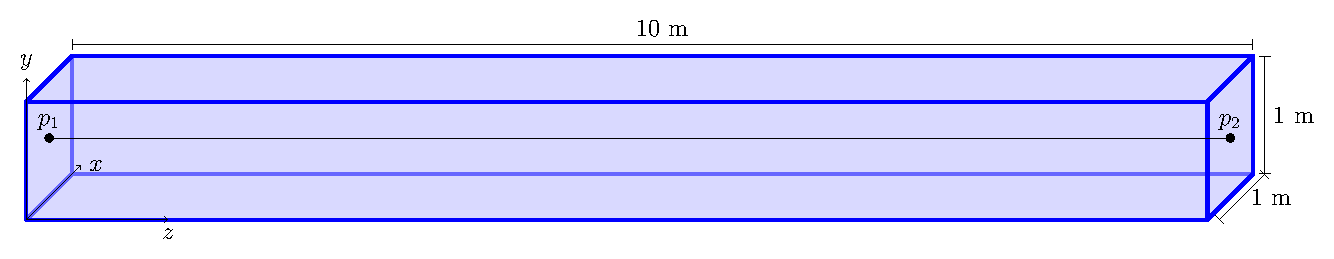
\includegraphics[page=1, width=\textwidth]{Figuras/viga_longa.pdf}
    \label{fig:viga_longa_geometria}
\end{figure}

\begin{figure}
    \centering
    \caption{Uma viga longa.}
    \includegraphics[page=2, width=\textwidth]{Figuras/viga_longa.pdf}
    \label{fig:viga_longa_condicoes}
\end{figure}

\begin{figure}
    \centering  
    \caption{Deformação na direção de $y$ ao longo da linha $\overline{p_1 p_2}$}
    \includegraphics[page=3, width=\textwidth]{Figuras/viga_longa.pdf}
    \label{fig:viga_longa_deslocamento}
\end{figure}


